\documentclass[10pt,landscape,a4paper, fleqn, dvipsnames]{article}
\usepackage[utf8]{inputenc}
\usepackage[ngerman]{babel}
\usepackage[T1]{fontenc}
%\usepackage[LY1,T1]{fontenc}
%\usepackage{frutigernext}
%\usepackage[lf,minionint]{MinionPro}
\usepackage{tikz}
\usetikzlibrary{shapes,positioning,arrows,fit,calc,graphs,graphs.standard}
\usepackage[nosf]{kpfonts}
\usepackage[t1]{sourcesanspro}
\usepackage{multicol}
\usepackage{wrapfig}
\usepackage[top=0.8cm,bottom=0.8cm,left=0.75cm,right=1cm]{geometry}
% \usepackage[top=1cm,bottom=1cm,left=0.75cm,right=1cm]{geometry} for pages 4
\usepackage[framemethod=tikz]{mdframed}
\usepackage{microtype}
\usepackage{pdfpages}
\usepackage{verbatim}
\usepackage{graphicx}

\usepackage{enumitem}
\setlist{nolistsep, leftmargin = 1em}
\setlist[2]{nolistsep, leftmargin = 1.5em}
% \setlist{nolistsep}
% \setlist{leftmargin = 1em}
\renewcommand{\labelitemii}{$\circ$}

\usepackage{xcolor}
% \usepackage[dvipsnames]{xcolor}
\definecolor{mygray}{rgb}{0.8,0.8,0.8}
\usepackage{listings}
\lstset{%
basicstyle=\ttfamily,
breaklines = true,
backgroundcolor=\color{mygray},
}
\usepackage{realboxes}
\usepackage{soul}
% \usepackage[fleqn]{amsmath}


\let\bar\overline

\include{inhalt/def}

\begin{document}
%\footnotesize

% \setlength{\abovedisplayskip}{0pt}
% \setlength{\belowdisplayskip}{0pt}
% \setlength{\abovedisplayshortskip}{0pt}
% \setlength{\belowdisplayshortskip}{0pt}

\small
\begin{multicols*}{3}
\section*{SMP and Gale Shapley}
\begin{itemize} %[itemsep=0ex,topsep=-2ex]
    \item instability: say $(m, w')$ is instable if 
    \begin{itemize}[leftmargin = 1em]
        \item $m$ prefers $w'$ more than his current $w$, and
        \item $w'$ prefers $m$ more than her current partner $m'$
    \end{itemize}
    \item note: the set S returned by GS is unique, even if 
    there's more than one perfect pairing
    \item runtime: $\Theta(n^2)$
\end{itemize}
    % insert Gale Shapley Code
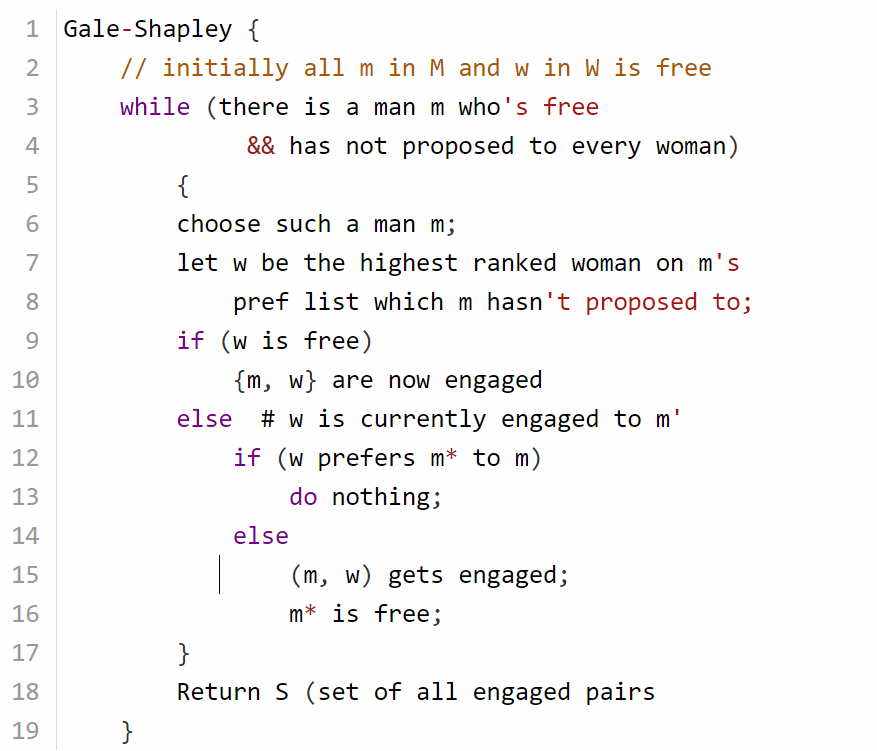
\includegraphics[scale = 0.61]{pictures/gale-shapley code.png}

    % \begin{verbatim}
    % Gale-Shapley {
    % // initially all m in M and w in W is free
    % while (there is a man m who's free 
    %          && has not proposed to every woman) 
    %     {     
    %     choose such a man m;
    %     let w be the highest ranked woman on m's 
    %         pref list which m hasn't proposed to;
    %     if (w is free)
    %         {m, w} are now engaged
    %     else  # w is currently engaged to m'
    %         if (w prefers m* to m) 
    %             do nothing;
    %         else 
    %             (m, w) gets engaged;
    %             m* is free;
    %     }
    %     Return S (set of all engaged pairs
    % }
    % \end{verbatim}

\section*{Runtime Analysis} % move the headers in a bit
\begin{itemize}
    % \item limit definitions \\
    % 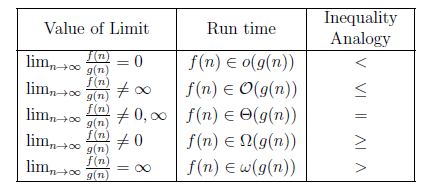
\includegraphics[scale = 1]{pictures/big o definition.png}
    \item big $O,~ \Omega,~ \Theta$ definition 
    \begin{align*}
        f &= O(g):~~\exists c, ~ \exists n_0~\text{ s.t }  n \geq n_0 \rightarrow f(n) \leq cg(n)\\
        f &= \Omega(g):~~ \exists c, ~\exists n_0 ~ \text{ s. t } n \geq n_0 \rightarrow f(n) \geq c g(n)\\
        &\rightarrow \text{ or } g \in O(f) \\
        f &= \Theta(g): ~~ f = O(g) \text{ and } f = \Omega(g)
    \end{align*}
    \item small $o, \omega$
    \begin{align*}
        f &= o(g): ~~ \forall c, ~ \exists n_0 ~ \text{ s.t } n \geq n_0 \rightarrow f(n) < c g(n) \\
        f &= \omega(g) ~~ \forall c, ~ \exists n_0 ~ \text{ s.t } n \geq n_0 \rightarrow f(n) > c g(n)
    \end{align*}
    \item small $o, \omega + \Theta$ limit definition
    \begin{align*}
        \lim_{n \rightarrow \infty} \frac{f(n)}{g(n)} = L~~
        \begin{cases}
            L = 0 \rightarrow f \in o(g) \\
            L = c \rightarrow f \in \Theta(g) \\
            L = \infty \rightarrow f \in w(g)
        \end{cases}
    \end{align*}
    \item big $O, \Omega$ limit definition
    \begin{align*}
        \lim_{n \rightarrow \infty} \frac{f(n)}{g(n)} = L ~~
        \begin{cases}
            L \neq \infty \rightarrow f \in O(g) \\
            L = \infty \rightarrow f \in \Omega(g)
        \end{cases}
    \end{align*}
    
    \item these are a list of common runtime (fastest $\rightarrow$ slowest in terms of runtime) 
    \end{itemize}
    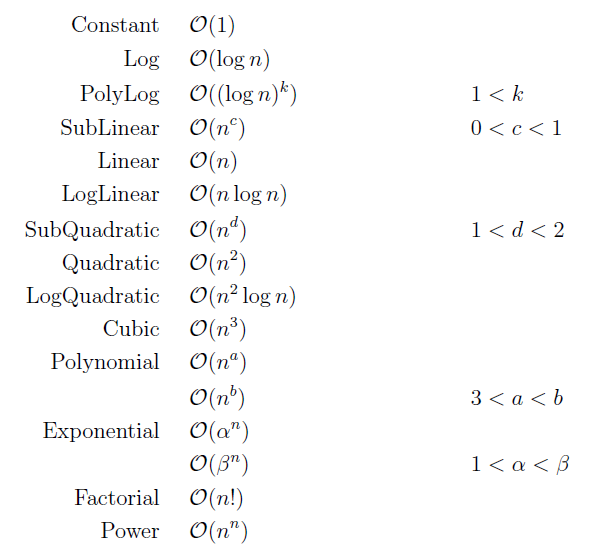
\includegraphics[scale = 0.7]{pictures/functions growth.png}
    \begin{itemize}
    \item important math/log rules
    \begin{align*}
        &c^{\log_c a} = a                   &&\log_a(x) > \log_b(x) \text{ if } a < b \\
        &\log_c (a \cdot b) = \log_c a + \log_c b           &&\log_c (b^k) = k \log_c b \\
        &\log_c (a / b) = \log_c a - \log_c b               &&\log_a b = {\log_c a}/{\log_c b}   \\
        % &&\log_c c = 1\\
        &C(n,r) = {n \choose r} = \frac{n!}{r!(n-r)!}              && P(n,r) = \frac{n!}{(n-r)!}
    \end{align*}
    % 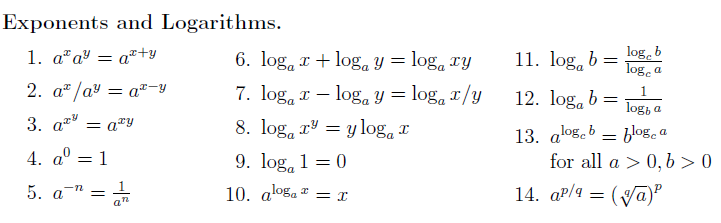
\includegraphics[scale = 0.7]{pictures/exponent and log.png}
    % \vfill\null 
    % \columnbreak 
    
\end{itemize}
\section*{Graphs}
\begin{itemize}
    \item \textbf{\ul{simple definitions}}
    \begin{itemize}[leftmargin = 1em]
    % \setlength{\itemindent}{-1.5em}
        \item path: sequence of verticies $\{v_1, v_2, \ldots, v_k\}$ s.t there exists an edge between consecutive vertices 
        \item simple path: a path that doesn't pass through any vertex more than once
        \item cycle: path w/ common beginning and ending (ex. $\{ v_1, v_2, \ldots, v_k \},~ v_1 = v_k$)
    \end{itemize}
    \item \textbf{\ul{types of graphs:}}
    \begin{itemize}[leftmargin = 1em]
    % \setlength{\itemindent}{-1.5em}
        \item simple: no self-edge and multi-edged vertices
        \item cyclic: graph got at least 1 cycle
        \item connected: every pair of distinct vertices has an edge b/t them 
        \item complete: every vertex has an edge to every other vertex in the graph
        \item tree: undirected. connected, acyclic graph 
        %insert some picture if have space
    \end{itemize}
    % \vfill\null \columnbreak
    \item \ul{\textbf{math for graphs}}: let graph $G = (V,E)$, $| V| = n $ and $|E| = m$ 
    \begin{itemize}[leftmargin = 1em]
    % \setlength{\itemindent}{-1.5em}
        \item simple graphs:
        \begin{align*}
            &\text{sum of degrees in G: } \small {\scriptstyle \sum} _{v \in V} deg(v) = 2m \\
            &\text{\# of edges in complete graph: } m = \frac{n}{2} (n-1)
        \end{align*}
        \item connected simple graph: $O(n) \subset O(m) \subset O(n^2)$ \\
        $\longrightarrow m \in O(n) \Longrightarrow $ graph is sparse \\
        $\longrightarrow m \in O(n^2) \Longrightarrow$ graph is dense 
        \item min \# of edges in connected graph: $m = n-1$
        \item max \# of edges in connected graph\\
        $\longrightarrow$ simple: $n(n-1)/2$ (complete graph)\\
        $\longrightarrow$ not simple: DNE
    \end{itemize} 
    \item topological ordering: all vertices line up in a way that all edges point forward (top. ordering might not be unique)
    % \item DAG: directed acyclic graph 
    % $\longrightarrow G$ is a DAG if it has a topological ordering ($\therefore$ DAG means no cycles
    \item \ul{\textbf{some propositions:}}
    \begin{itemize}[leftmargin = 1em]
    % \setlength{\itemindent}{-1.5em}
        \item any pair of v's in a \ul{tree}, there's a path that connects them
        \item any graph w/ n vertices and n edges has a cycle
        \item let $G$ be an undirected graph w/ $n$ vertices, if any of the following 2 is True, all 3 is True
        \begin{enumerate}
            \item G is connected
            \item G is acyclic
            \item G has $n-1$ edges
        \end{enumerate}
    \end{itemize}
    \item basic graph function runtime\\
        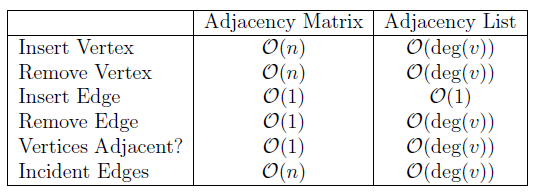
\includegraphics[scale = 0.8]{pictures/runtime graph basic.png} 
\end{itemize}
% \newpage
\subsection*{Search Algorithm}
\begin{itemize}
    \item \ul{\textbf{runtime for graph searching algorithms}} \\
    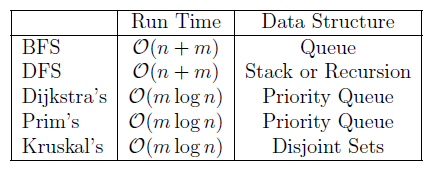
\includegraphics[scale = 0.9]{pictures/runtime graph algo.png}
    \item Prim's and Krushkal's are used to find MST in a weighted graph (can handle negative edges)
    \item Dijkstra's used to find shortest path between two nodes in a weighted graph (cannot handle negative edges)
    \item \textbf{Note}: heights of BFS \& DFS nodes depends on start node and order nodes are checked
    \vfill\null \columnbreak
    \item BFS
    \begin{itemize}[leftmargin = 1em]
        \item uses a queue $\rightarrow$ explores the graph in layers
        \item used to find the shortest path from $s$ to all $v \in V$
    \end{itemize}
    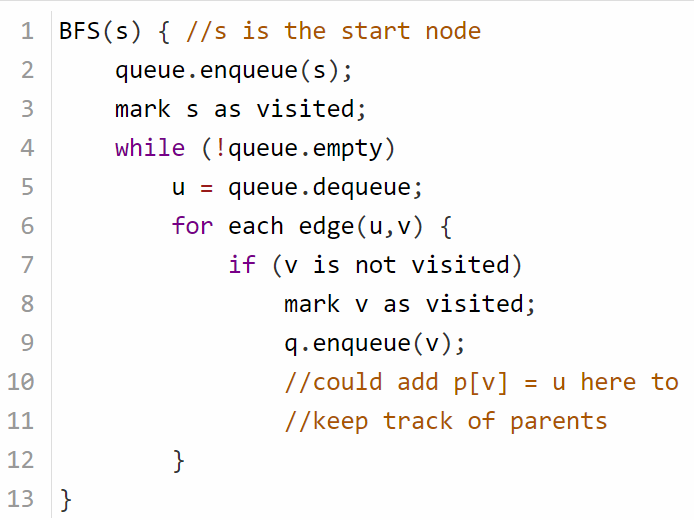
\includegraphics[scale = 0.6]{pictures/BFS code.png} 
    \item DFS
    \begin{itemize}[leftmargin = 1em]
        \item uses a stack/recursion
        \item explores the point further from the graph first
        \item does not find the shortest path 
        \item can identify cycles
    \end{itemize}
    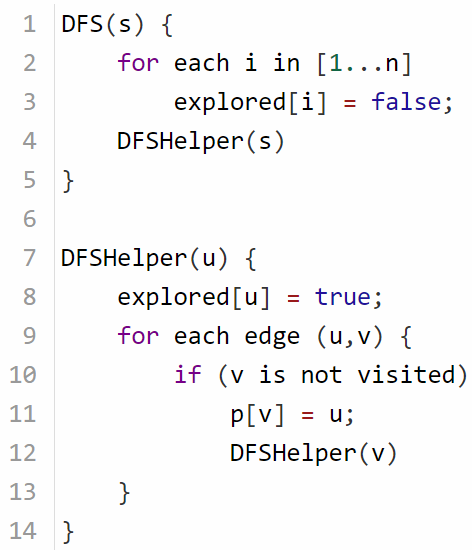
\includegraphics[scale = 0.6]{pictures/DFS code.png}
   
\end{itemize}

% do Greedy proofs too if you have time
\section*{Divide and Conquer}
\begin{itemize}
    \item Summations and Geometric Series 
    % \\
    % 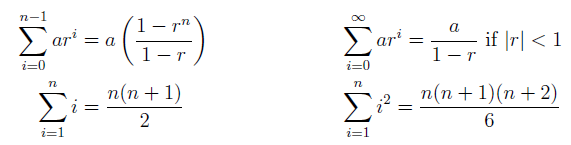
\includegraphics[scale = 0.75]{pictures/summation.png}
\end{itemize}
{\color{Violet}
\begin{align*}
    \sum^{n}_{i=1} a r^i &= a \left(\frac{1-r^n}{1-r} \right) = a\cdot   \frac{r^{n+1}-1}{r-1}
    &&\sum_{i=0}^\infty ar^i = \frac{a}{1-r} ~~~ \text{ if } |r| < 1 \\
    \sum^n_{i=1} i &= \frac{n(n+1)}{2} 
    &&\sum^n_{i=1}i^2 = \frac{n(n+1)(n+2)}{6}
\end{align*}
}
\begin{itemize}
    \item \ul{\textbf{The Master Theorem}}
    {\color{Violet}
    \begin{align*}
        T(n) &= 
        \begin{cases}
            c~ \text{ (has to be constant)} &\text{if } n < n_0 \\
            aT\left(\frac{n}{b} \right) + cn^k &\text{if } n \geq n_0
        \end{cases} \\
        \text{if } a > b^k &: T(n) \in \Theta(n ^{\log_b a}) \\
        \text{if } a = b^k &: T(n) \in \Theta(n^k \log n) \\
        \text{if } a < b^k &: T(n) \in \Theta(n^k)
    \end{align*}
    }
    $\rightarrow$ Master theorem does not always give same bound as tree
    \item let tree be $T(n) = a T(n/b) + cn$, then $height(tree) = \log_b n$
    \item some divide and conquer algo w/ their runtime\\
    $\longrightarrow$ quickSort: $\Theta(n\log n )$\\
    $\longrightarrow$ quickSelect (find k-th largest element in array): $\Theta(n)$
    \item find work per level: get work at level one in form of $cn^k \cdot (a/b)$ and the work per level is $cn^k(a/b)^i$
    \item if you can't use Master theorem (unequal split) - 2 ways 
    \begin{itemize}[leftmargin = 1em]
        \item \ul{\textbf{massage into Master Theorem}}: 
            \begin{align*}
                T(n) &= T\left( \frac{3n}{4} \right) + T \left(\frac{n}{8} \right) + cn \\
                \text{define } L(n) &= T \left(\frac{n}{8} \right) + T \left(\frac{n}{8} \right) + cn \leq T(n) \\
                &= 2T \left(\frac{n}{8} \right) + cn  \\
                U(n) &= 2 T \left(\frac{3n}{4} \right) +cn \geq T(n) \\ 
                \text{via Master, } L(n) &= \Theta(n) \therefore T(n) = \Omega(n) \\ 
                U(n) &= \Theta(n) \therefore T(n) = O(n) \\
                \therefore T(n) &= \theta(n)
            \end{align*}
        \item \ul{\textbf{take sum to infinity}}: the lower bound is the work done at level 0, and upper bound is sum of work done per level take to infinity 
        \begin{itemize}[leftmargin = 1em]
            \item usually give tighter bound than the Master Theorem
            \item ex. $T(n) = 2T(n/3) + T(n/4) + cn^2$ for $n > 3$, constant other wise \\
            Work done at level 0: one root node of size n with time $cn^2$ \\
            Work done at level 1:
            \[c(n/3)^2 + c(n/3)^2 + c(n/4)^2 = cn^2(41/144)\] 
            Work per level: $cn^2 \cdot (41/144)^i$ \\
            Lower bound: work done at level 0 so lower bound is $ \Omega(cn^2)$\\
            Upper bound: 
            \begin{align*}
                \sum^\infty_{i=1} cn^2 \left(\frac{41}{144} \right)^i &= \dfrac{cn^2}{1-\frac{41}{144}} = cn^2 \left(\frac{103}{144} \right) = O(n^2)
            \end{align*}
        \end{itemize}
        
    \end{itemize}
\end{itemize}


\section*{Dynamic Programming}
The following example will use the Fibonnaci sequence 
\begin{align*}
    F(n) = 
    \begin{cases}
        1 & \text{ if } n \leq 2 \\
        F(n-1) + F(n-2) &\text{ if } n > 2
    \end{cases}
\end{align*} 

\begin{enumerate}
    \item Recursion
        \begin{itemize}[leftmargin = 1em]
            \item is pretty shit in terms of run time
        \end{itemize}
    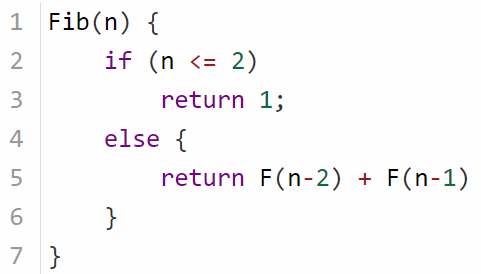
\includegraphics[scale = 0.6]{pictures/fibonacci recursion.png}
    \item Top-down Memoization
    \begin{itemize}[leftmargin = 1em]
        \item store past calls/results to memory
        \item needs helper $\rightarrow$ in helper check if it's been computed yet, usually means checking if the entry is 0 or $-1$
    \end{itemize}
    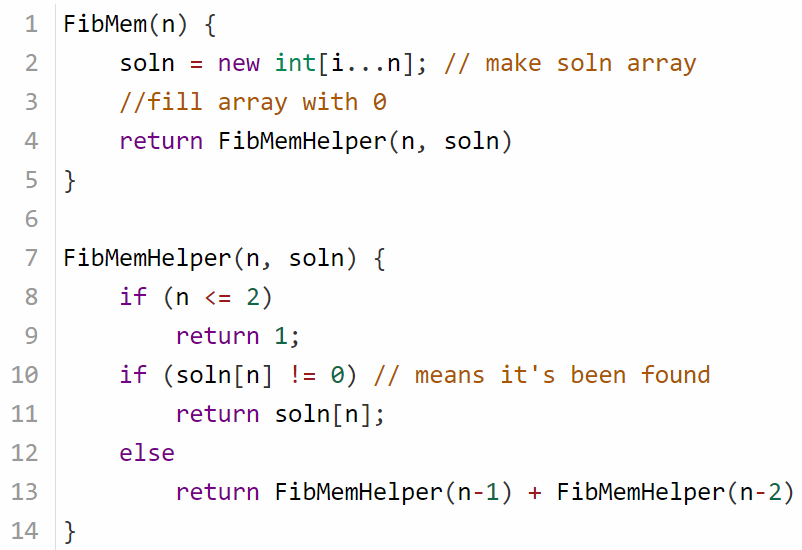
\includegraphics[scale = 0.6]{pictures/fibonacci memoized.png}
    \item Dynamic Programming (Bottom-Up)
        \begin{itemize}[leftmargin = 1em]
            \item calculate all necessary entries first
            \item use for loop $\rightarrow$ usually code inside for loop is direct translation of recurrence relation
        \end{itemize}
    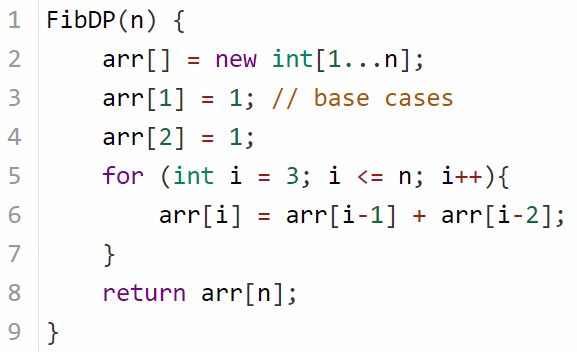
\includegraphics[scale = 0.6]{pictures/fibonacci dp.png}
\end{enumerate}
\begin{itemize}
    \item making change problem: give the minimum number of change for a dollar amount - imagine all possible coins are \$0.25, \$0.10, and \$0.01. 
\end{itemize} 
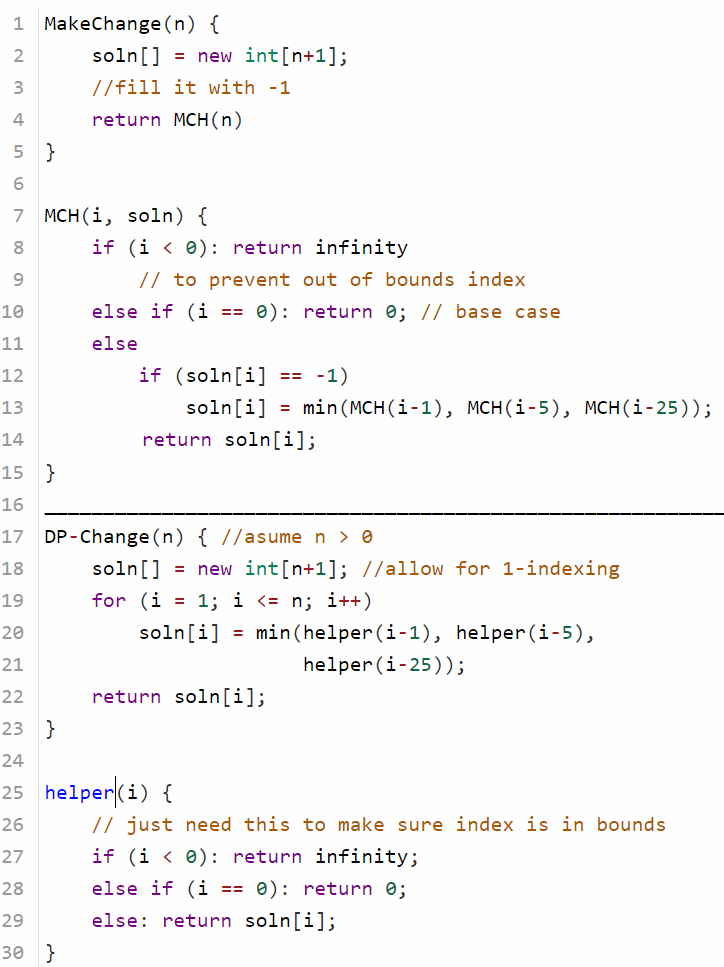
\includegraphics[scale = 0.7]{pictures/Change code.png} 
\begin{itemize}
    \item \ul{\textbf{runtime}}
    \begin{itemize}[leftmargin = 1em]
        \item recursion: see how many recursive call is called per iteration (call $a$), and how deep the recursive call (call $b$) - get $a^b$, multiply that with time for the base case
        \begin{itemize}[leftmargin = 1em]
            \item ex. Fibonacci: 2 recursive call, each getting called n times $r\rightarrow 2^n$ factor and base case is $O(1)$ - so total runtime is $O(2^n)$
        \end{itemize}
    
        \item Memoization \& DP: think about how much work you're doing without recursive call and then think about how many (non-repetitive) recursive call you're making, then calculate the total 
        \begin{itemize}[leftmargin = 1em]
            \item thinking about it in terms of for loops and DP makes a bit more sense
            \item ex. Fibonacci: Work without recursive call is $\Theta(1)$. Number of unique recursive call is $\Theta(n)$. So total is $\Theta(n)$ 
        \end{itemize}
    \end{itemize}
    \vfill \null \columnbreak
    \item tips - when identifying sub problems
    \begin{itemize}[leftmargin = 1em]
        \item if problem involve discrete quantities then sub problem would be about smaller quantities $\rightarrow$ going backwards - likely memoization
        \item if problem is going forward (computing the next value or seeing if going forward in 1 direction gives the max/min - i.e midterm scheduling q) $\rightarrow$ likely DP
    \end{itemize}
\end{itemize}


\section*{NP Complete}
\begin{itemize}
    \item decision problem: problem that could be posed as yes no question - need to convert optimization problems into yes/no problems for NP proof\\
    $\longrightarrow$ "maximizing ..." $~=$ "... with size of at least $k$" \\
    $\longrightarrow$ "minimizing ..." $~=$ "... with size of at most $k$"
    \item let $\textbf P$ denotes set of decision problems where there's a known polynomial time algorithm
    \item efficient certifiers: an algo B is an efficient certifier for problem X if it can take a possible result and verify if it satisfy X in poly time
    \item let $\textbf{NP}$ denote set of problems for which we do not know if there's a poly-time algorithm. An algorithm X is in NP if there's an efficient certifier for it 
    \item \textbf{NP-Complete} are questions in NP but not P. So we don't know if there's an efficient algo. A decision problem X is in \textbf{NP-Complete} if: 
    \begin{itemize}[leftmargin = 1em]
        \item $X \in NP$, and
        \item $ Y \leq_p X,~ \forall Y \in NP$ (generalized to any (one) $Y \in NP$) 
        \item $Y \leq_p X$ means that there's a poly-time reduction from Y to X, or "X is at least as hard as Y"
    \end{itemize}
    \item it's obvious that $\textbf {P } \subseteq \textbf{ NP}$
    \item if $Z \leq_p Y$ and $Y \leq_p X$, then $Z \leq_p X$
    \item if $Y \leq_p X$ and $X \in P$, then $Y \in P$\\
    $\longrightarrow$ if $Y \leq_p X$ and $Y \not \in P$, then $X \not \in P$ (contrapsitive)
    \item \textbf{NP-Hard}: like NP-Complete but you drop the first requirement, you don't know it's in NP, just that it can be reduced from a problem in NP
    \item steps to NP-Complete proof
    \begin{enumerate}
        \item Show that there exist an efficient certifier for X (if answer is yes, then there's a proof of this fact that can be verified in P)
        \item Pick a known NP-Complete problem Y and specify how to reduce Y to X 
        \item Prove that reduction is correct \\
        $\longrightarrow$ meaning (yes instance in Y $\Longleftrightarrow$ yes instance in X)
    \end{enumerate}
    \item \textbf{\ul{aside - recall Bipartite Graph}:} A graph is Bipartite if you can partition $V$ into $V_1$ and $V_2$ such that there are no adjacent edges in $V_1$ and no adjacent edges in $V_2$ (likewise, if vertices are adjacent, they're in different sets). 
    \begin{itemize}[leftmargin = 1em]
        \item graph is bipartite if it's 2-colorable and has no odd cycles
    \end{itemize}
\end{itemize}
% \vfill \null\columnbreak
\subsection*{Important Problems}
The following pairs of NP-complete problems are of type $\{$\textcolor{teal}{\textbf{packing}}, \textcolor{Bittersweet}{\textbf{covering}}, \textcolor{Blue}{\textbf{partitioning problems}}, \textcolor{Magenta}{\textbf{sequencing}}, \textcolor{ForestGreen}{\textbf{numerical}}$\}$
%maybe colour code these%
\begin{itemize}
    \item \textcolor{teal}{\textbf{\ul{Independent Set}}}: For a graph $G = (V,E)$, a subset of vertices $S \subseteq V$ is independent if no vertices in S are joined by any edge. \ul{Given a graph $G$ and $k \in \mathbb{N}$ does $G$ contain an independent set of size $k$ or larger }
    \item \textcolor{teal}{\textbf{\ul{Set Packing}}}: Given an $n$-element set $U$,  a collection of subsets $\{S_1, S_2, \ldots, S_m \} \subset U$ and $k \in \mathbb{N}$, does there exists a collection of at least $k$ of those sets with property that no two of them intersect
    %insert set packing example here
    
    \item \textcolor{Bittersweet}{\textbf{\ul{Vertex Cover}}}: For a graph $G = (V, E)$, a subset of vertices $S \subseteq V$ is a vertex cover if every edge $e \in E$ has at least one endpoints in S. \ul{Given a graph $G$ and $k \in \mathbb{N}$, does G contain a vertex cover of size $k$ or smaller}
    %insert vertex cover and independent set example here
    \item \textcolor{Bittersweet}{\textbf{\ul{Set Cover}}}: Given an $n$-element set $U$, a collection of subsets $\{S_1, S_2, \ldots, S_m\} \subset U$ \& a number $k$, is there a collection of at most $k$ of those sets whose union is equal to U.
    
    \item \textcolor{Blue}{\textbf{\ul{3D Matching}}}: Given 3 disjoint sets, $X, Y, Z$, is there a set $T \subseteq X \times Y \times Z$ such that each elements of $U \cup Y \cup Z$ is contained exactly once in these triples
    \begin{itemize}[leftmargin = 1em]
        \item ex. $X = \{\text{instructors}\}, Y = \{\text{courses}\}, Z = \{\text{time slots}\}$
        \item is a special case of Set Cover, we're looking to cover the ground set $U = X \cup Y \cup Z$ using at most $n$ sets from $X \times Y \times Z$ 
        \item is a special case of Set Packing, since we're looking for $n$ disjoint subsets of ground set $U = X \cup Y \cup Z$
        \item Bipartite Matching (aka 2D matching): Given 2 Bipartite sets $U$ and $V$ find the maximum matching
        \begin{itemize}[leftmargin = 1em]
            \item ex. $U = \{readers\}, V = \{books\}$ and $(u,v)$ is book $v$ person $u$ willing to read $\rightarrow $ solve in $O(mn)$ time
        \end{itemize}
    \end{itemize}
    \item \textcolor{Blue}{\textbf{\ul{Graph Coloring}}}: A graph $G = (V,E)$ is said to be k-colorable if the endpoints of any edges $(u,v)$ can be coloured using diff colors when there's $k$ available colours. \ul{Given a graph $G$ and $k$, does $G$ have k-coloring?} 
    \begin{itemize}
        \item proof of NP-completeness is reduced from 3-SAT $\rightarrow$ that's why 2-colorable $\in P$
    \end{itemize}
    
    \item \textcolor{Magenta}{\textbf{\ul{Hamiltonian Cycle}}}: A simple cycle is a cycle in a graph with no repeated vertices (a cycle is permutation $\{v_1, v_2, \ldots, v_n \}$ with a pair $v_j = v_k$ but $j \neq k$. \ul{Given an undirected graph $G = (V,E)$, can you a simple cycle that visits every node $v \in V$}
    \item \textcolor{Magenta}{\textbf{\ul{Traveling Salesman}}}: A tour is a path that starts at city $C_1$ and visits every city exactly once and ends at $C_1$ again. \ul{Given a set of $ \{C_1, C_2, \ldots, C_n\}$, with list of costs where $c_{ij}$ of traveling from $C_i$ to $C_j$ and a number $k$, is there a tour with costs at most $k$}
    
    \item \textcolor{ForestGreen}{\textbf{\ul{Subset Sum}}}: Given a set of natural number $V = \{v_1, v_2 \ldots, v_n\}$ and a number $k$. Is there a subset $U \subseteq V$ such that sum of $U$ equals $k$?
    \item \textcolor{ForestGreen}{\textbf{\ul{Set Partition}}}: Given a set of $n$ integers $V = \{v_1, v_2, \ldots, v_n\}$, can elements of $V$ be partitioned into two sets $U$ and $(U-V)$ such that $\sum_{u \in U} u_i = \sum_{u \in (V-U)} u_i$?
    
    \item \textcolor{BrickRed}{\textbf{special, 3-SAT}}: all clauses are of length 3 with $n$ literals, of the form below. \ul{Given a SAT instance, could you create a truth assignment $T = \{t_1, t_2, \ldots, t_n\}, ~ t_i \in \{0, 1\}$} that satisfies the instance \\
    $\longrightarrow \text{ ex. } (x_1 \lor \bar x_2 \lor x_3) \cap (x_4 \lor x_5 \lor x_6)$\\
    $\longrightarrow$ 2-SAT $\in P$
    \item \textcolor{BrickRed}{\textbf{special, clique}}: For a graph $G = (V, E)$, a subset of vertices $S \subseteq V$ is a clique if every pair of vertices in V is joined by an edge (so find a complete subgraph basically). \ul{Given a graph $G$ and $k$, does $G$ contain a clique of size at least $k$?}
    \item \textbf{\ul{note}}: 3-SAT $\leq$ Independent Set $\leq$ Vertex Cover $\leq$ Set Cover
\end{itemize}


\subsection*{Example Reduction}
\subsubsection*{Independent Set $<_p $ Vertex Cover}
\ul{\textbf{1. Vertex Cover $\in$ NP}} \\
Given a solution set $S$, for every vertex in $S$, delete all adjacent edges from the graph's edge set $E$. At the end, if $E$ is empty, it was a vertex cover. If we use adjacency lists, runtime is $O(m) \subseteq O(n^2)$ - \medskip so it's in poly-time, thus vertex cover $\in$ NP. \\
\ul{\textbf{2. Reduction}}: \\
From diagram below, we can see that independent set and vertex cover problems are complements of each other. So for a graph $G = (V,E)$ with $n$ vertices, and independent set $S$ of size $k$ produces and vertex cover of $(V - S)$ of size $n - k$. So no changes necessary \medskip for the graph itself, just pass $k' = n - k$ into \Colorbox{mygray}{\lstinline|VertexCover(G, k)|}\\
\ul{\textbf{3. Proposition}}: Set $S$ is an independent set iff its complement $V - S$ is a vertex cover\\
\ul{$\Longrightarrow:$} Proceed by contradiction and suppose $S$ is an independent set, yet $V -S$ is not a vertex cover. That means there's an edge $e = (u,v) \in E$  such that neither endpoints are in $(V-S)$ - so $u,v \not \in (V-S)$. But then that means that $u, v \in S$, but then $S$ is not an independent set. $\blacksquare$ \\
\ul{$\Longleftarrow$:} Proceed by contradiction and suppose $(V-S)$ is a vertex cover, but $S$ is not an independent set. So there must be an edge $e = (u,v) \in E$ such that both $u,v \in S$. But that means that $u, v \not \in V-S$, so $e$ is an edge with no end point in $(V-S)$ and so $(V-S)$ is not a vertex cover. $\blacksquare$


\subsubsection*{Hamiltonian Path $\leq$ The Traveling Salesman}
\ul{\textbf{1. TSP $\in$ NP}}\\
Given a possible solution set of vertices $S$, check that $S$ is a tour by removing every $v \in S$ from $V$ (if $v \in V$, if $v \not \in V$ that means that we've traveled to that city twice, reject) and that $(v_i, v_{i+1}) \in E$. We can also keep track of total cost of every $(v_i, v_{i+1}) \in S$ At the end, $V$ should be empty and the sum of cost should be $k$. We could check \medskip all this in $O(n)$ so TSP $\in$ NP. \\
\\
\ul{\textbf{2. The Reduction}}\\
For an instance $G = (V, E)$ with $|V| = n$ of \Colorbox{mygray}{\lstinline|HamCycle|}, we'll make a new instance $I_G$. In $I_G$, we'll turn every node $i \in V$ to corresponding cities $C_i$ in \Colorbox{mygray}{\lstinline|TSP|}. We then can create edges between all cities (make a complete graph, not a requirement in TSP but for our case we want this) make set the weights of $(C_i, C_j) = 1$ if $(i, j) \in E$, otherwise, the cost is 2. We also set the new $k' = n$ (set it to $n$ because we want to reach every node) and feed that into TSP. Creating a new list of cities can be done in $O(n)$ time and if we're using adjacency lists for the edges, we can set all edges to 2 in $O(n^2)$ and change all edges that exist in $E$ to 1 in also $O(n^2)$ times. So total time of \medskip reduction is $O(n^2)$ \\
\ul{\textbf{3. Proposition:}} Show that your reduction is correct, that is $G$ is a Yes-instance of HamCycle iff $I_G$ is a Yes-instance of TSP\\
\ul{$\Longleftarrow$}: Suppose that $I_G$ is a Yes-instance of TSP, so there's a tour of the cities that cost at most $k = n$. Let $\{C_{i1}, C_{i2}, \ldots, C_{in}\}$ be successive cities on this tour. Then the cost is 1 to get from any city to the next conseuctive city in the tour, and also the cost is 1 to get back from the last to the first (if any of the cost was 2, the total would be at least $n+1$). The reduction forces the fact that inter-city costs are 1 iff there's an edge in $E$ between the corresponding nodes in $G$, so $E$ must contain $(i_n, i_1)$ as well as $(i_j, i_{j+1})$ for $1 \leq j \leq n-1$. So if we take the corresponding nodes, the permutation $\{i_1, i_2, \ldots, i_n\}$ is a Hamiltonian cycle of $G$ and $G$ is a Yes-instance \\
\ul{$\Longrightarrow$}: Suppose G is a Yes-instance, with Hamiltonian cylce $i_1, i_2, \ldots, i_n$. Then the reduction guarantees that Cities $C_{i1}, C_{i2}, \ldots, C_{in}$ form a tour where the cost from one city to the next is 1, and the cost of getting back from the last city to the first is also 1. So, $I_G$ has a tour of cost $n$ and so is a Yes-instance of the TSP problem 


% \subsubsection*{Subset Sum $\leq$ Set Partition}
% \ul{\textbf{1. Set Partition $\in$ NP}} \\
% Given sets $A$ and $B$, to check that they are partitions of $U$, we need to check $A \cup B = U$, $A \cap B = \varnothing$ and $\sum_{a_i \in A} a_i = \sum_{b_i \in B} b_i$. To check first requirement (the union), add $A$ and $B$ to a set and check if that's equal to $U \longrightarrow$ would take $O(n\log n)$ because need to sort the sets to compare. For the second, put elements of $A$ into hashsets and check every element of $B$ to see if it's already in there. Thirdly, we can compute the sum as we go along doing the last step $\longrightarrow$ both these things take $O(n)$. So checking takes $O(n\log n) \subset O(n^2)$. Thus \medskip Set Partition $\in $ NP.\\
% \ul{\textbf{2. The Reduction}} \\
% The intution is that for a set $V$, $\sum_{v_i \in V} v_i = s \in \mathbb{Z}$. If we successfully partition $V$ into $U$ and $U-V$, then $\sum_{u_i \in U} u_i = \sum_{u_i \in (V-U)} u_i = s/2$. Then, if we wanted it look for a partition that sum to $k$, we need all elements in V to sum to $2k$ - can do this by adding a integer $t$ to $V$ with value $(2k-s)$. \\
% So, given a set $V$, for a set $V' = V \cup \{2k-s\}$ and feed $V'$ into \Colorbox{mygray}{\lstinline|SubsetCover(V)|}. This will return 2 subsets, both of which sum to $k$, pick the one without $2k-s$. The reduction takes polynomial \medskip time because you're just adding an element.\\
% % insert picture 
% \ul{\textbf{3. Proposition}}: Let $V = \{v_1, v_2, \ldots, v_n\}$ and $k \in \mathbb{Z}$. \textbf{Prove that an instance is Yes instance in the Subset Sum problem iff it's a Yes instance in Set Partition} \\
% \ul{$\Longrightarrow$}: Suppose that $I$ is a Yes-instance in \Colorbox{mygray}{\lstinline|SubsetSum|}. This means that there's a subset $W \subseteq V$ such that $\sum_{w_i \in W} w_i = k$. Let $\sum_{v_i \in V} v_i = s \in \mathbb{Z}$ and let $V' = V \cup \{2k - s\}$, we will feed $V'$ into \Colorbox{mygray}{\lstinline|SetPartition|}. Consider sets $W$ and $V' - W$, we need to show that these 2 sets are the partition of $V'$ that will give us the right answer. \\
% First, we have $W \cup (V' - W) = V'$ and $W \cap (V' - W) = \varnothing$ via definition of complement. Since $\sum_{v'_i \in V'} v'_i = s + (2k-s) = 2k$ and $\sum_{w_i \in W} w_i = k$, this must mean $\sum_{w_i \in (V'-W)} w_i$. Therefore, we have $\sum_{w_i \in W} w_i = \sum_{w_i \in (V'-W)} w_i$ as required. So we have a Yes instance in \Colorbox{mygray}{\lstinline|SetPartition|} as well. $\blacksquare$ \\
% \ul{$\Longleftarrow$}: Suppose there's a partition of $V'$, $U$ and $V' - U$. Because of the nature of $V'$ and set partition, we know $\sum_{u_i \in U} u_i = \sum_{u_i \in (V' - U)} u_i = k$. We also have the fact that they are disjoint, so $2k -s$ belongs to just one of the sets. WLOG, assume that set is $V'-U$, then $U$ is the subset of $V$ that we're looking for. And so we have a Yes instance in \Colorbox{mygray}{\lstinline|SubsetSum|} as well


% we want less spaces between items
\end{multicols*}
\end{document}